\chapter[Modeling approach for realistic simulation of online reprocessing]{Modeling approach for realistic simulation of online reprocessing}

\section{Reprocessing plant general concept}
Removing specific chemical elements from a molten salt is a complicated 
task that requires intelligent design (e.g., chemical separations 
equipment design, fuel salt flows to equipment) and has a considerable 
economic cost. This section contains a brief overview of general 
chemical processing plant and a gas separation system. As an example 
of generic reprocessing facility the reprocessing plant of a single-fluid 
\gls{MSBR} was selected.

\subsection{Gas separation system}
Volatile gaseous fission products (e.g. Kr, Xe) must be removed from the fuel salt 
to avoid reactor poisoning especially during starup and power maneuvering. This is 
particularly true for $^{135}$Xe, with its very large neutron capture cross 
section (2.65$\times$10$^6$ b). Conceptually, tritium, xenon, and krypton 
can be removed from the fuel salt by helium bubbles introduced in a stream 
by a bubble generator and subsequently removed 
by a gas separator (figure~\ref{fig:gas_removal_system}). Indeed, noble gases, because of their exceptional insolubility 
in the salt, will migrate promptly to any gaseous interface available. Because 
they form an ideal-dilute mixture in salt (obey Henry's law), they will migrate in 
accordance with the conventional laws of mass transfer. If tiny helium bubbles 
are circulated with the fuel salt, they will absorb xenon and krypton fission 
products. The fission-product-rich bubbles of helium may then be separated from 
the salt and discharged to the off-gas system. Xenon migration to the circulating 
bubbles competes with xenon migration to the porous moderator graphite. 
The graphite is especially of concern because it absorbs xenon and holds it in the 
core which leads to parasitic neutron absorption. The 0.5\% target value for 
$^{135}$Xe poison fraction can be achieved when circulating helium bubbles are 
0.508mm in diameter \cite{robertson_conceptual_1971}. This is accomplished by 
redirecting 10\% of the fuel salt flow from the pump discharge 
through a bubble separator 
to remove the xenon bubbles and then back into the pump suction. The average 
residence time of a bubble in the fuel loop would be 10 full cycles. Investigation 
for the \gls{MSBR} has shown that helium babble size was approximately 25\% of the 
throat width (blue circle on figure~\ref{fig:bubble_separator}) and was independent 
of the gas flow rate \cite{robertson_conceptual_1971}. Consequently, it is possible 
to regulate helium bubble size by changing throat width in the bubble generator.
\begin{figure}[htp!] % replace 't' with 'b' to 
  \centering
  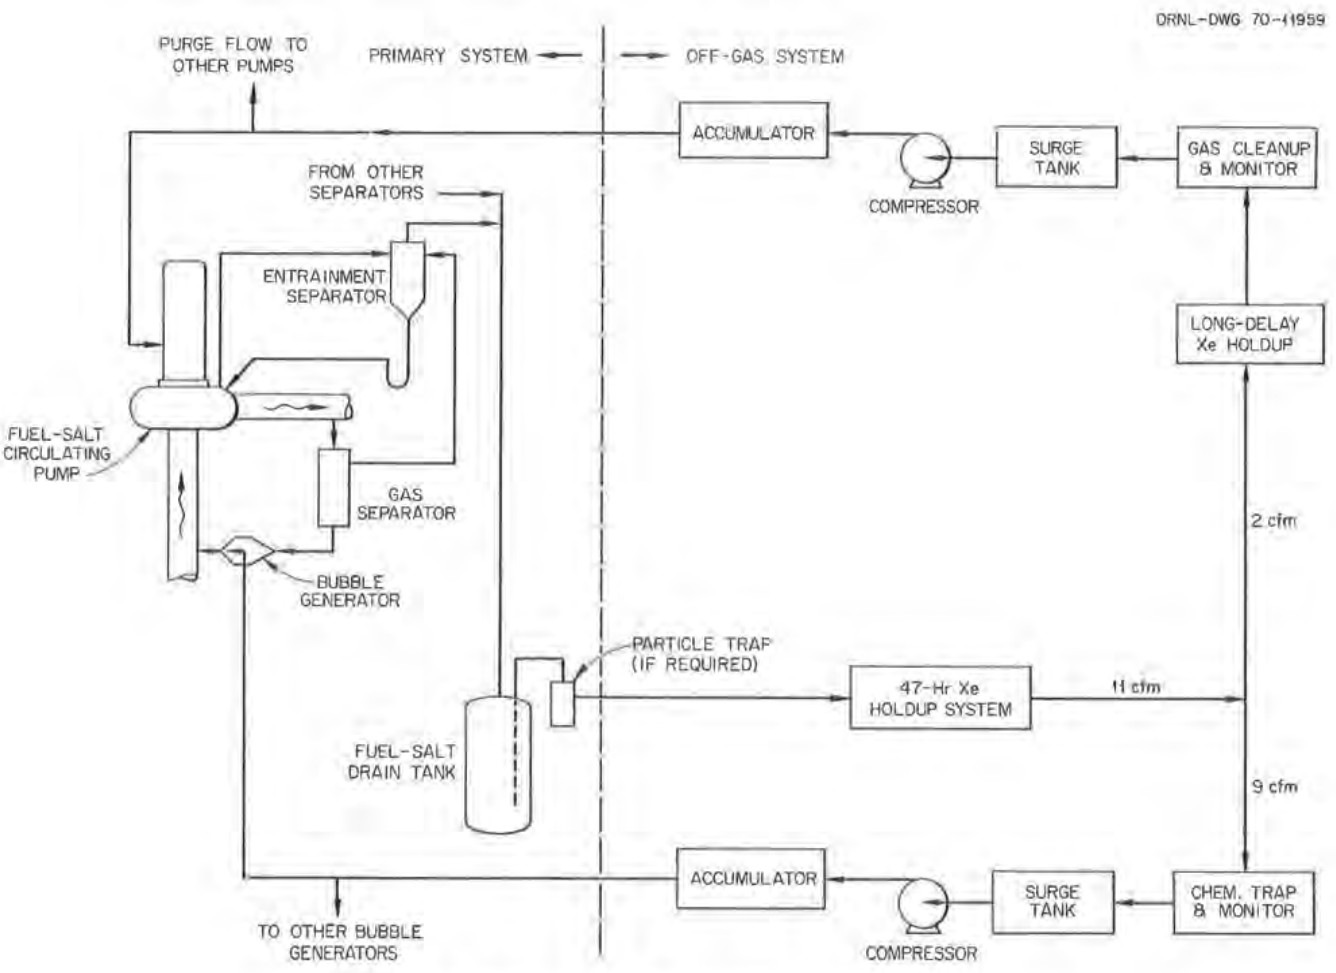
\includegraphics[width=\textwidth]{gas_separation.png}
  \caption{Schematic flow diagram of the \gls{MSBR} off-gas system (figure 
  reproduced from Robertson \emph{et al.} \cite{robertson_conceptual_1971}).}
  \label{fig:gas_removal_system}
\end{figure}
\begin{figure}[htp!] % replace 't' with 'b' to 
  \centering
  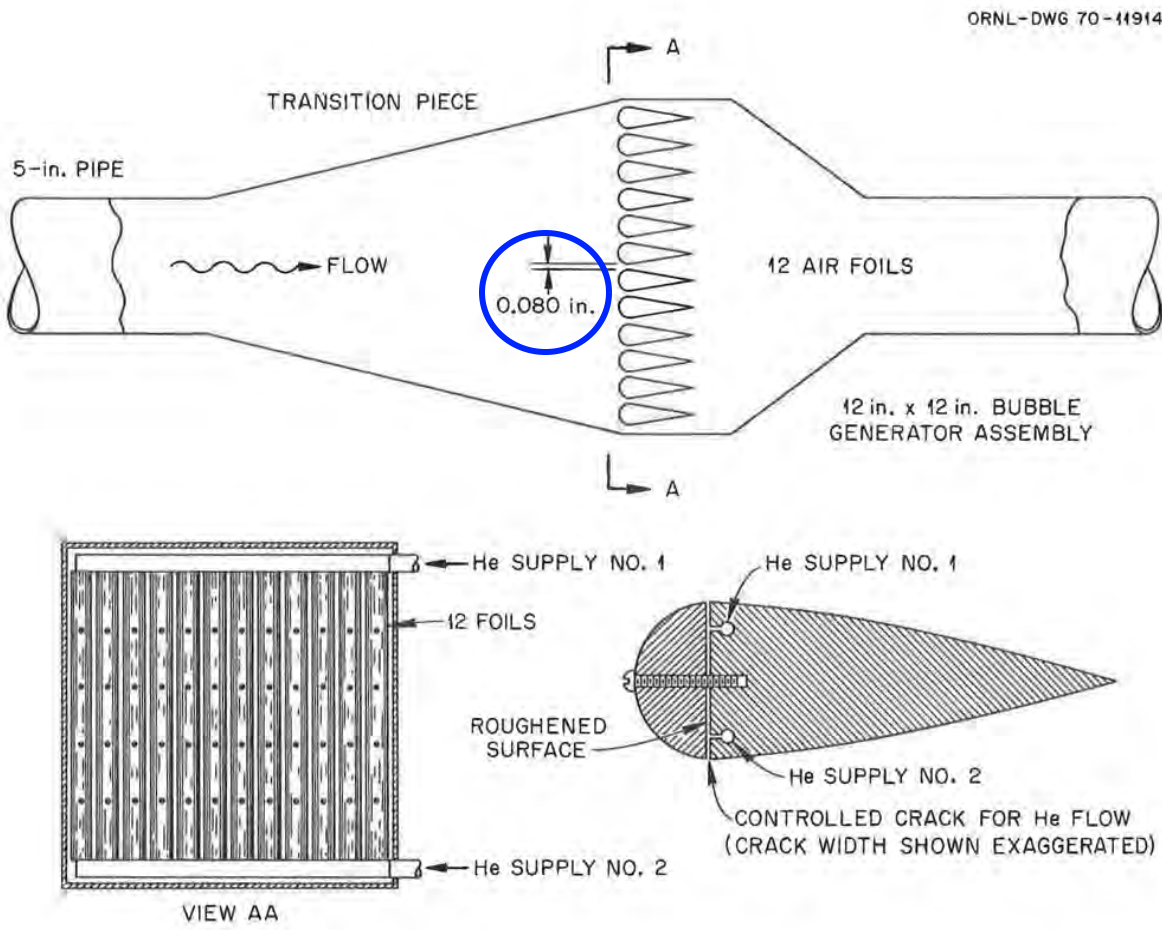
\includegraphics[width=\textwidth]{msbr_bubble_generator.png}
  \caption{Preliminary concept of \gls{MSBR} bubble generator (figure 
  reproduced from Robertson \emph{et al.} \cite{robertson_conceptual_1971}). 
  The blue circle shows 
  throat width, which determines bubble size.}
  \label{fig:bubble_separator}
\end{figure}

To inform physics-based, numerical simulation of volatile gas removal 
a mathematical model is required. Particularly, a model of xenon extraction 
efficiency as a function of sparger design parameters is needed to accurately 
model $^{135}$Xe removal in a fuel salt 
depletion simulations. The gain and loss terms for $^{135}$Xe dissolved in the fuel 
salt are listed in tables~\ref{tab:xe_gain} and \ref{tab:xe_loss}. 
The stripping efficiency for the pump bowl has been measured during the \gls{MSRE} but 
the \gls{ORNL} report only states its range (from 50 to 100\%) and mentioned that the 
results are not accurate \cite{kedl_development_1967}. $^{135}$Xe burnup and 
decay rates are well known. The mass transfer coefficient for transferring xenon into 
helium bubbles can be estimated from CFD-models but published information is 
insufficient to inform an accurate mathematical model. 
Previous research by \gls{ORNL} \cite{kedl_development_1967, engel_xenon_1971} has 
concluded that xenon removal efficiency ($\epsilon_{Xe}$) in a gas separation 
system is a function of many parameters:
\begin{align}
& \qquad\qquad\qquad\qquad\qquad \epsilon_{Xe} = F (A, d_{He}, \dot{m}_{He}, \dot{m}_{salt}, h_b, T)
	\intertext{where}
 	A      &= \mbox{the interface area of the injected helium bubbles} \nonumber \\
 	d_{He} &= \mbox{the average diameter of helium bubbles} \nonumber \\
 	\dot{m}_{He} &= \mbox{the helium gas mass flow rate} \nonumber \\
 	\dot{m}_{salt}&= \mbox{the salt mass flow rate} \nonumber \\
 	h_b &= \mbox{the mass transfer coefficient for transferring xenon into circulating helium bubbles} \nonumber \\
 	T &= \mbox{the salt temperature} \nonumber
\end{align}
\begin{table}[ht!]
\caption{$^{135}$Xe production sources and principal rate constants involved
 (reproduced from Kedl \emph{et al.} \cite{kedl_development_1967}).}
  \centering
\begin{tabularx}{\textwidth}{b | b}
\hline \textbf{$^{135}$Xe gain mechanism}      & \textbf{Principal rate 
parameters involved}  	\\
\hline Direct from Fission   & (Fission rate) $\times$ 0.3\% (for $^{235}$U fission) \\
\hline $^{135}$I decay       & (Fission rate) $\times$ 3.6\% (for $^{235}$U fission) \\
iodine-135 generation rate is 3.6\%, 
it decays to $^{135}$Xe with $\tau_{1/2}=6.68$ h & 			                    \\		\hline $^{135}$Te decay      & (Fission rate) $\times$ 2.5\% (for $^{235}$U fission) \\
tellurium-135 generation rate is 2.5\%, 
it quickly decays to $^{135}$I with $\tau_{1/2}=19$ s & 			                    \\					
\hline 
\end{tabularx}
  		\label{tab:xe_gain}
\end{table}
\begin{table}[ht!]
\caption{$^{135}$Xe loss terms and principal rate constants involved
 (reproduced from Kedl \emph{et al.} \cite{kedl_development_1967}).}
  \centering
\begin{tabularx}{\textwidth}{b | b}
\hline \textbf{$^{135}$Xe loss mechanism}      & \textbf{Principal rate 
parameters involved}  	\\
\hline Decay of dissolved $^{135}$Xe ($\tau_{1/2}=9.1$ h)  & Decay constant	($\lambda$)		\\
\hline $^{135}$Xe burnup              &  Neutron flux ($\Phi$)		 					\\
dissolved xenon-135 burnup as it passes throught core  & 			            \\		\hline $^{135}$Xe transferred to off-gas system via xenon stripper & Stripping efficiency ($\epsilon$)		\\
\hline $^{135}$Xe transferred into circulating He bubbles; this xenon will eventually be burnup, decay, or stripped via bubble separator & Mass transfer coefficient ($h$), decay constant ($\lambda$), 
neutron flux ($\Phi$), bubble removing efficiency ($\epsilon$)		\\
\hline 
\end{tabularx}
  		\label{tab:xe_loss}
\end{table}

This technique would be applicable to other noble gases (e.g. Kr) but the 
correlation coefficients are different. 
To create a realistic mathematical model, correlations with 
coefficients for various volatile gases (particularly xenon) are needed. These 
correlations can be obtained experimentally or using CFD simulations. 
Current efforts at the University of Illinois at Urbana-Champaign namely, ``Enabling 
Load Following Capability in the Transatomic Power MSR" \cite{huff_enabling_2018}, 
have a goal to determine those correlations using CFD simulations 
and verify it in small-size experiments. 
As a result, the obtained mathematical model might be used to inform realistic 
physics-based gas removal from fuel salt in the proposed SaltProc tool.

\subsection{Fuel salt chemical processing facility} \label{sec:chemical_processing}
In the single-fluid \gls{MSBR}, thorium, uranium, 
protactinium, and fission products are all mixed together in a single fluoride salt (FLiBe). The \gls{MSRE} demonstrated a liquid-liquid extraction process 
for removing protactinium and uranium from molten fluoride salts. The method 
is to exchange thorium and lithium dissolved in molten bismuth for the 
components to be removed from the salt. Moreover, the \gls{MSRE} reports 
indicated that the extraction could be carried out rapidly and continuously 
\cite{whatley_engineering_1970-1}.

The principal scheme of the \gls{MSBR} reprocessing facility concept is shown in Figure~\ref{fig:material_flow}. The fuel salt is first temporarily stored for cooling and decay of the shortest lived fission products, then directed to the primary fluorinator where most of the uranium is removed by fluorination to UF$_6$. After that, the salt is routed to an extraction column where mixture containing metallic bismuth, lithium and thorium as reductants are contacted with the salt. The remaining uranium and protactinium are reductively extracted to a bismuth solution, leaving a salt that only contains fission products dissolved in carrier salt (base composition LiF-BeF$_2$-ThF$_4$). The salt then goes through a reduction column where UF$_6$ is reduced to UF$_4$ in the salt and preparing it for return to the reactor. Refill BeF$_2$ and ThF$_4$ are also added and all residual bismuth is removed from the salt. After a final cleanup step and valence adjustment, the purified salt returns to the reactor \cite{carter_design_1972,sorensen_one-fluid_2006}.
\begin{figure}[htp!] % replace 't' with 'b' to 
  \centering
  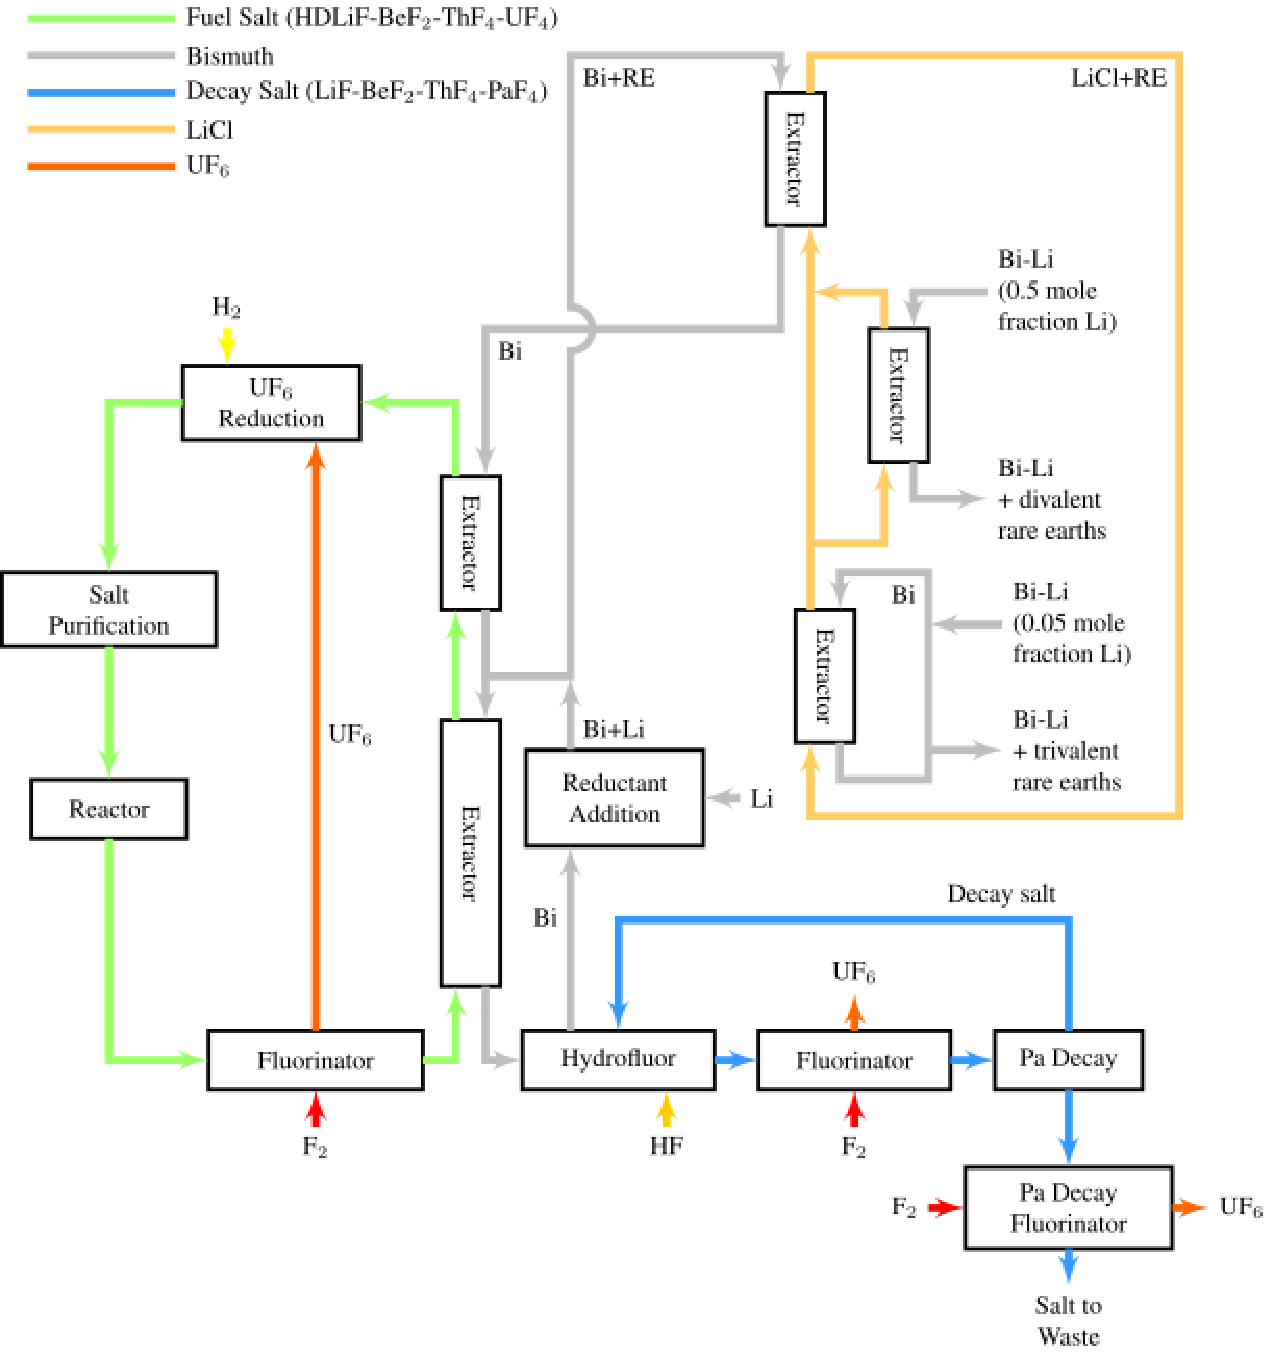
\includegraphics[width=0.9\textwidth]{flowsheet.pdf}
  \caption{Simplified block diagram of chemical processing scheme for single-fluid \gls{MSBR} (reproduced 
  from Sorensen \cite{sorensen_one-fluid_2006}). RE is a reducing agent.}
  \label{fig:material_flow}
\end{figure}

The bismuth binding to uranium and protactinium is routed to a hydrofluorination column where the metallic solutes in the bismuth are oxidized into their fluoride forms in the presence of a decay salt\footnote{The decay salt contains UF$_4$, PaF$_4$, ThF$_4$ and fission products. Uranium produced after $^{233}$Pa decay is extracted and directed back into the reactor. Decay salt is the precursor for the waste salt as it was periodically discarded every 220 days.}. The decay salt, containing UF$_4$, PaF$_4$, and ThF$_4$ passes into a decay tank where $^{233}$Pa is decays to $^{233}$U. The uranium generated by protactinium decay is removed through fluorination to UF$_6$ and directed to the reduction column to refuel the purified fuel salt. A hydrofluorinator and a fluorinator can remove approximately 95\% of the uranium from the stream 
\cite{robertson_conceptual_1971}.

The fully processed salt, on its way back to the reactor, has uranium added from the protactinium decay tank at the rate required to maintain or adjust the uranium concentration in the reactor (and, consequently, control the reactivity). Adding fissile material are performed by sparging the salt with UF$_6$ and hydrogen to produce UF$_4$ in the salt and HF gas \cite{robertson_conceptual_1971}.

The fuel salt stream from the protactinium isolation system contains only traces of protactinium and uranium (because it was separated in the system) but contains practically all of the rare earths. A fraction of this salt stream is redirected to a reductive extraction process for removing rare earths.  The principal scheme of a rare earth removal system is shown in Figure~\ref{fig:rare-earth-removal}. A molten salt flow which contains rare-earth fluorides is fed to the center of an extraction column. The salt flows countercurrent to a liquid bismuth stream which contains thorium and lithium. In the upper part of the column, the rare earths are reduced and transferred to the downflowing liquid metal stream. Below the feed point, the rare earth concentration is increased in the salt and metal streams in order to produce a concentration high enough for disposal \cite{briggs_molten-salt_1969}.

Molten salt leaving the top of the column contains a dilute concentration of rare earths. A fraction of this flow is returned back to the reactor while the rest is sent to an electrolytic cell complex. The net effect of the complex is to push thorium and lithium into bismuth and to return extracted rare earths, entering the complex with bismuth from the bottom of the cascade, to the cascade as reflux, oxidizing them out of the metal and transferring them to the returning salt stream.
\begin{figure}[htbp!]
  \centering
        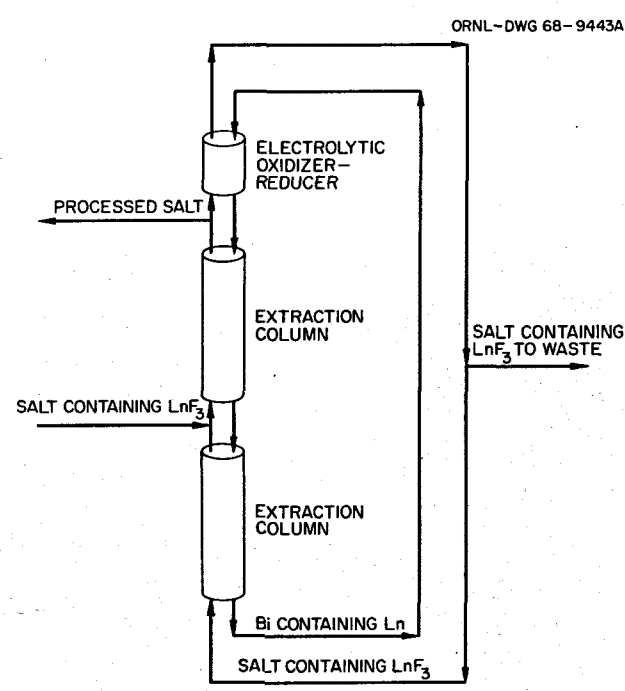
\includegraphics[width=0.45\textwidth]{rare-earths-removal-system.png}
    \caption{Rare earth removal from a fuel salt by reductive extraction (figure 
    reproduced from Briggs \emph{et al.} \cite{briggs_molten-salt_1969}).}
    \label{fig:rare-earth-removal}
\end{figure}

\subsection{Rare Earths Separation Efficiency} \label{sec:rare_earth_eff}
Rare earth removal efficiencies were calculated during Molten Salt Reactor Experiment for a range of operating conditions to establish the importance of number of stages, separation factor\footnote{Separation factor is ratio of target element (e.g. promethium) concentration in metal phase (e.g. Li-Bi) to target element concentration in the salt.}, metal-to-salt flow ratio, rare earth concentration in the discard stream, location of the feed point, and the fraction of ThF$_4$ which is reduced in the electrolytic oxidizer-reducer. The thorium and lithium concentrations in the bismuth stream fed to the extraction column were both 0.0016 mole fraction. 
\begin{figure}[htbp!]
    \begin{center}
        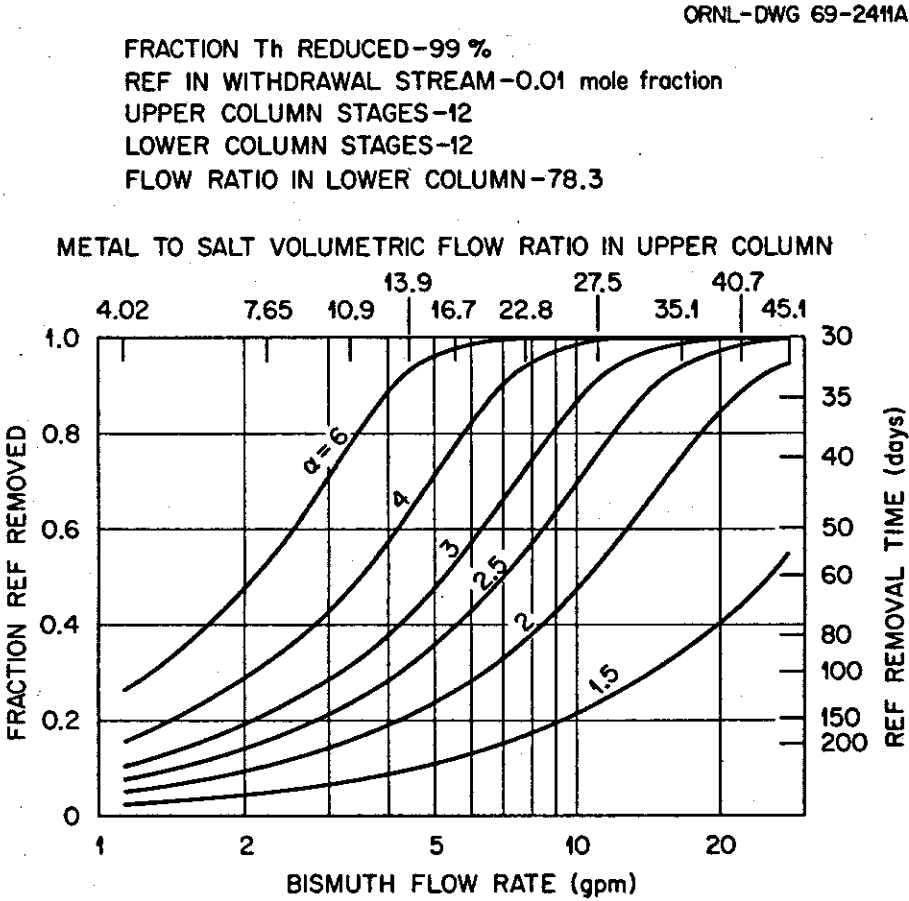
\includegraphics[width=0.55\textwidth]{vol_flow_ratio.png}
    \end{center}
    \caption{Metal-to-salt volumetric flow ratio in upper column (24-stage column) \cite{briggs_molten-salt_1969}.}
    \label{fig:vol-flow-ratio}
\end{figure}

The optimum feed location was at the center of the column and all results herein is for this feed
location. System performance is shown in Figure~\ref{fig:vol-flow-ratio} for a range of metal-to-salt flow ratios and for rare-earth-thorium separation factors from 1.2 to 6. The fraction of the ThF$_4$ which is reduced in the electrolytic cell was 99\%. Operation with a bismuth flow rate of 15 gpm will result in a rare earth removal efficiency of 69\% (44-day removal time) for a separation factor of 2 and a removal efficiency of 31\% (95-day removal time) for a separation factor of 1.5.

The effect of fraction of ThF$_4$ reduced in the electrolytic cell is shown in Figure~\ref{fig:th-reduction}. A significant decrease in removal efficiency results from the fraction of ThF$_4$ reduced being decreased from 99 to 90\%, and the system becomes ineffective if less than 50\% of the ThF$_4$ is reduced.  The separation factors are 1.3 for Eu, 1.7 for Pm, 1.8 for La, 2.0 for Sm, 3.0 for Nd, and 3.5 for Ce. The removal times range from about 225 days for Eu to 30 days for Nd and Ce (Table~\ref{tab:removal_time}). 
\begin{figure}[htbp!]
  \centering
        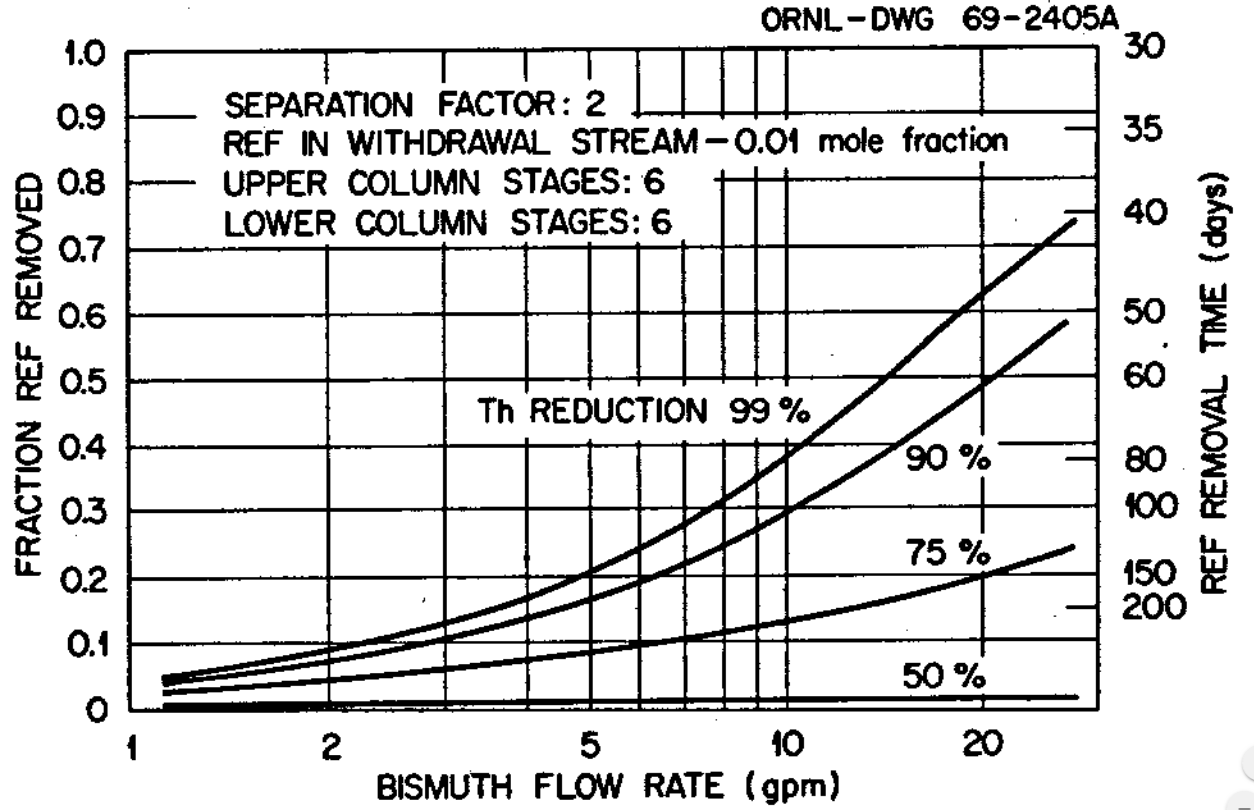
\includegraphics[width=0.55\textwidth]{th_reduction.png}
    \caption{Rare earth removal system performance as function of bismuth phase flow rate and the thorium removal in the electrolytic cell complex (figure reproduced from Briggs \emph{et al.} \cite{briggs_molten-salt_1969}).}
    \label{fig:th-reduction}
\end{figure}
\begin{table}[ht!]
\caption{Removal cycle times for various rare earths \cite{briggs_molten-salt_1969}.}
  \centering
\begin{tabular}{c c c}
\hline Rare  & Separation & Removal Time                        \\
       Earth & Factor     & (days)								\\
\hline Pm          & 1.7				& 63.8 					\\
\hline Nd		   & 3.0                & 30.6 					\\
\hline Sm		   & 2.0                & 43.5 					\\
\hline La		   & 1.8                & 47.7 					\\
\hline Eu		   & 1.3                & 222.0 				\\
\hline Ce		   & 3.5                & 30.3 					\\
\hline 
\end{tabular}
  		\label{tab:removal_time}
\end{table}

Promethium, one of the rare earths, determines the operating conditions for the removal system (Pm has a separation factor of 1.7), since it is the strongest neutron absorber. Lanthanum is less important, and the resulting removal time ($\approx$100 days) is satisfactory.
The removal times for rare earths having separation factors greater than 2, such 
as neodymium and cerium, will be shorter than required.

Overall, based on experimental data from the \gls{MSRE}, chemistry-based mathematical models can be formulated for rare earths separation efficiency. 
The analysis above 
shows that the efficiency of specific rare earth removal ($\epsilon_{RE}$) 
in a chemical processing plant is a function of many parameters:
\begin{align}
& \qquad\qquad\qquad  \epsilon_{RE} = F (A, \dot{m}_{Bi}, \dot{m}_{salt}, N, K)
	\intertext{where}
 	A &= \mbox{a metal-to-salt interface area} \nonumber \\
 	\dot{m}_{Bi} &= \mbox{the bismuth mass flow rate} \nonumber \\
 	\dot{m}_{salt}&= \mbox{the salt mass flow rate} \nonumber \\
   	N &= \mbox{the number of stages} \nonumber \\
 	K &= \mbox{the mass transfer coefficient at the salt / Bi-Li interface} \nonumber
\end{align}
These mathematical correlations can be used to inform realistic chemistry-based 
depletion simulations with the proposed SaltProc tool.

\section{SERPENT overview}
SERPENT is a continuous-energy Monte Carlo neutronics software capable of solving the neutron transport problem by tracking individual neutrons within the problem geometry and using stochastic method to determine chain of events for each neutron \cite{leppanen_serpent_2015}. SERPENT has been under active development at the VTT Technical Research Centre of Finland since 2004, where it was initially conceived as a tool to simplify group constant generation in a high-fidelity Monte Carlo environment. SERPENT is now widely used transport code  with a growing user base. Now SERPENT used by more than 500 registered individuals in 155 organizations located in 37 countries around the world. The burnup calculation capability in SERPENT is based on built-in calculation routines, without using any external solvers. A restart feature allows performing fuel shuffling or applying any modifications in the input by dividing the calculation into several parts, which is crucial for online reprocessing simulations.

The latest version, SERPENT 2, supports advanced geometries and has advanced burnup capabilities, including online refueling capabilities which are necessary for neutronic computations of pebble-bed reactors and liquid-fueled \glspl{MSR} \cite{aufiero_extended_2013}. Unfortunately, built-in online refueling features are still under active development and unavailable to ordinary users. Furthermore, recently multi-physics simulations using SERPENT 2 were demonstrated, including  calculations with thermal-hydraulics, \gls{CFD} and fuel performance codes \cite{leppanen_numerical_2015}. Two-way coupling to thermal-hydraulics, \gls{CFD}, and fuel performance codes operates on two levels: internal coupling to built-in solvers for fuel behavior and thermal-hydraulics and external coupling via a universal multi-physics interface. 

SERPENT 2 can be effectively run in parallel on computer clusters and multi-core workstations. Parallelization is handled by thread-based OpenMP, which enables all processsors to use shared memory space. Calculations can be divided into several nodes by distributed-memory \gls{MPI} parallelization. SERPENT 2  is an improvement upon SERPENT 1, and contains a complete redesign of memory management using hybrid OpenMP \cite{dagum_openmp_1998} + \gls{MPI} parallelization.  This hybrid parallelization is important in depletion calculations using computer clusters with multiple nodes, and allows to achieve significant speed-up in depletion calculations on computer clusters with more than 4'000 cores \cite{leppanen_serpent_2015}. 

All calculations herein were performed using SERPENT 2 version 2.1.30 on Blue Waters’ XE6 nodes. For cross section generation, the JEFF-3.1.2 nuclear data library was employed based on entirely open cross section data 
\cite{oecd/nea_data_bank_jeff-3.1.2_2014}. 

\section{Proposed simulation tool design and capabilities} \label{sec:tool_design}
The first version of the SaltProc Python tool for calculating \gls{MSR} fuel 
composition evolution taking into account an online reprocessing system 
was developed as a part of my M.Sc. thesis \cite{rykhlevskii_advanced_2018,
rykhlevskii_arfc/saltproc_2018}. The tool was designed to 
expand SERPENT 2 depletion capabilities for modeling liquid-fueled \gls{MSR} 
for online reprocessing. SaltProc uses HDF5 
\cite{the_hdf_group_hierarchical_1997} to store 
data and uses the PyNE Nuclear Engineering Toolkit \cite{scopatz_pyne_2012}
for SEPRENT output file parsing and nuclide naming. SaltProc is an 
open-source Python package that uses a batch-wise approach to simulate 
continuous feeds and removals in \glspl{MSR}. 

Capabilities of the developed tool, working with the Monte Carlo software 
SERPENT 2, were demonstrated using the full-core MSBR design for a 
simplified case with ideal removal efficiency (100\% of mass for target 
elements removed) \cite{rykhlevskii_modeling_2019}. Unfortunately, 
the code architecture and principal structure was not designed for 
flexible implementation of sophisticated online reprocessing systems 
including realistic physics/chemistry-based extraction efficiencies. 
Thus, complete refactoring of SaltProc using \gls{OOP} is needed to 
create a comprehensive generic tool to realistically model any \gls{MSR} 
reprocessing plant while taking into account variable extraction 
efficiencies, mass balance between the core and processing plant and 
reactivity control system.

\subsection{Proposed software architecture}
The SaltProc v2 Python toolkit will couple directly with SERPENT 2 input 
and output files, 
to allow the reprocessing system to couple to depletion calculation. 
Existing PyNE interfaces will be employed for SERPENT 2 output parsing as 
well as newly developed interfaces for input and output handling. 
Python 3 \gls{OOP} 
standard features will be used to create a flexible, user-friendly tool with 
great potential for further improvement and collaboration. 
Figure~\ref{fig:saltproc_class} shows the proposed SaltProc class structure 
 which includes 4 main classes:
\begin{enumerate}
	\item \textit{Depcode}. Contains attributes and methods for 
	reading the user's input file for the depletion software, initial 
	material (e.g., fuel and/or fertile salt) composition, principal 
	parameters for 
	burnup simulation (e.g., neutron population and number of cycles for Monte 
	Carlo), running the depletion code. The proposed work will only 
	support SERPENT 2 Monte Carlo (only 
	one instance of \textit{Depcode} will be instantiated) but in principle the 
	toolkit can support any depletion code (i.e. OpenMC 
	\cite{romano_openmc_2015}).
\begin{figure}[ht!] % replace 't' with 'b' to \centering
  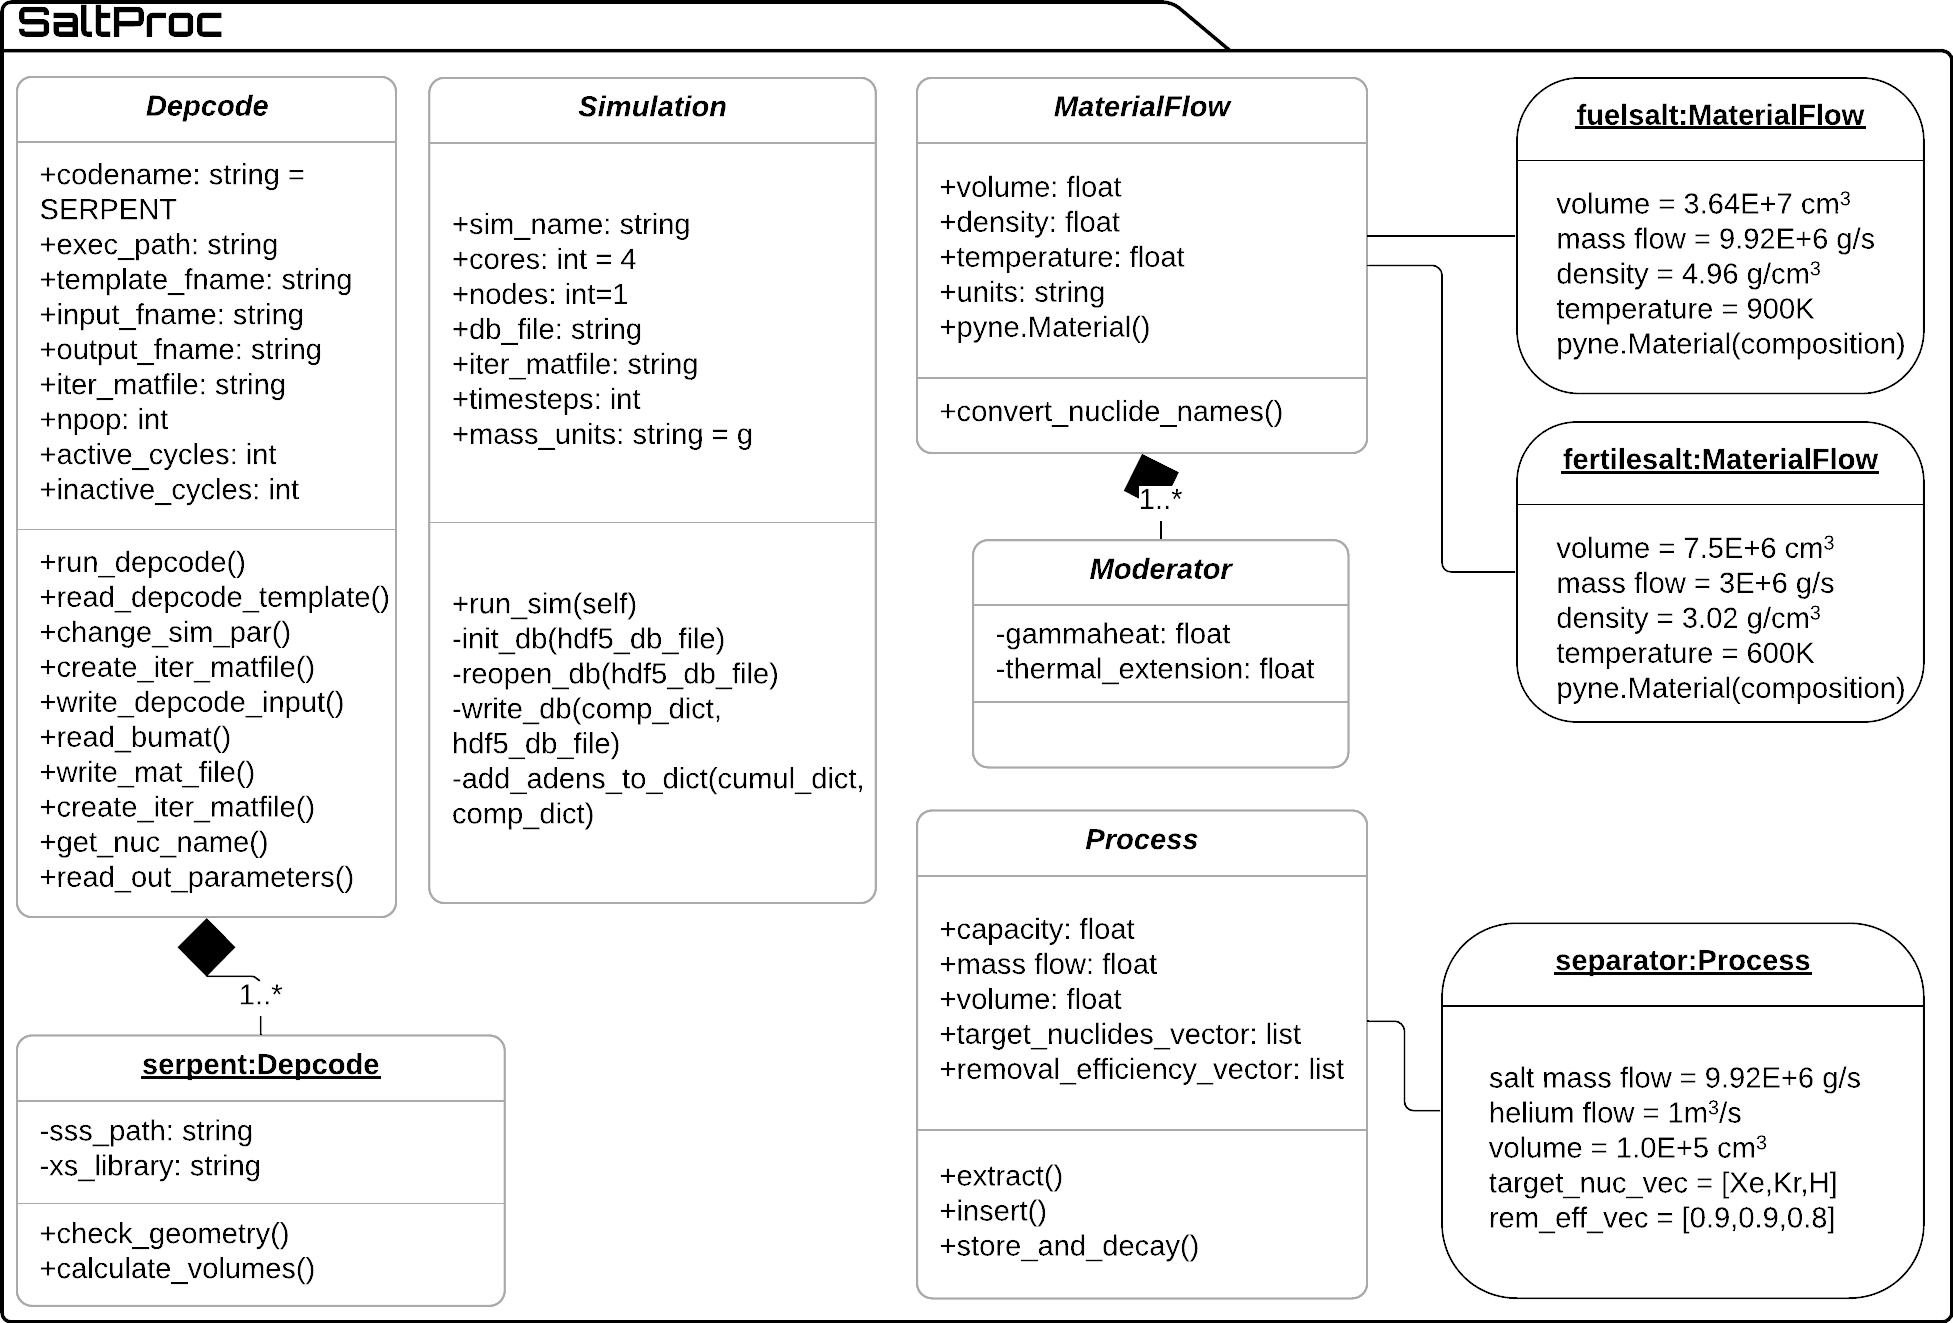
\includegraphics[width=\textwidth]{saltproc_class_diagram.png}
  \caption{Saltproc python package tentative class diagram with UML notation 
  and examples of object instances.}
  \label{fig:saltproc_class}
\end{figure}
	\item \textit{Simulation}. Runs SaltProc simulation step, 
	create, write HDF5 database, track time and convert 
	isotopic composition vector nuclide names from SERPENT to human 
	readable format. Also this class will allow simulation restart after 
	failure by restoring data from the HDF5 database and continue simulation 
	for additional depletion time.
	
	\item \textit{MaterialFlow}. Each \textit{MaterialFlow} object 
	will represent the material flowing between \textit{Process} objects. 
	The object of this class will contain an isotopic composition vector 
	(PyNE Material object 
	initialized	from SERPENT output file \textbf{dep.m}), mass flow rate, 
	temperature, density, volume, and void fraction. Existing PyNE Material 
	capabilities allows on to easily convert the units of isotopic 
	composition vector (e.g., from atomic density provided by SERPENT to 
	mass fraction or absolute mass in desired units), decay material 
	(i.e. model the \gls{MSBR} protactinium decay tank), calculate 
	decay heat, activity and dose. The main idea of the \textit{MaterialFlow} 
	object is to pass detailed information about the salt starting at the 
	\gls{MSR} vessel outlet throughout reprocessing facilities 
	(\textit{Processes}), which are modifying the \textit{MaterialFlow} 
	object before depleting the material in the next SERPENT burnup step.
		
	\item \textit{Process}. Each \textit{Process} object will represent a 
	realistic fuel processing step characterized by its throughput rate, 
	volumetric capacity, extraction efficiency for each target element (can be 
	function of many parameters), waste streams, and other parameters specific to 		the particular process. Refueling 
	\textit{Process} injects feed \textit{MaterialFlow} usually directly 
	into the reactor core (e.g., adding fissile material with specific mass flow 		rate to \textit{MaterialFlow} after performing all removals).
\end{enumerate}

The proposed class structure will provide outstanding flexibility in simulating 
various \gls{MSR} designs. A library of various \textit{MaterialFlow} (e.g., 
fuel salt flow, fertile salt flow, refueling salt flow) and \textit{Process} 
(e.g., helium sparging facility, gas separator, lanthanide removal component) 
objects will be created in this work to allow a user to quickly create a model 
of a desired reprocessing scheme. At runtime, the user will connect 
\textit{Process} objects in series or parallel with \textit{Flow} objects to 
form a comprehensive reprocessing system. The user will also be able to create 
a custom object with desired attributes and methods, and contribute back 
to the code package using Github (https://github.com/arfc/saltproc).	

\subsection{Tentative flowchart}
Figure~\ref{fig:saltproc_flow} illustrates the online reprocessing simulation 
algorithm coupling SaltProc and SERPENT 2. To perform a depletion step, 
SaltProc reads a user-defined SERPENT 2 template file. This file contains input 
 parameters such as geometry, material, isotopic composition, neutron 
population, criticality cycles, total heating power, and boundary conditions.  
After the depletion calculation, SaltProc reads the depleted fuel composition 
file and stores the depleted composition isotopic vector in an HDF5 database 
and \textit{MaterialFlow} object (\textit{CoreOut} in 
figure~\ref{fig:saltproc_flow}). This object contains an isotopic composition 
vector, total volume of material, mass flow rate, density and any other 
parameters specified by user. For the simplest reprocessing case, when all 
facilities are located in-line (100\% of total material flow goes through 
chain of separation components), the \textit{CoreOut} object is flowing 
sequentially between \textit{Processes} and each \textit{Process} is 
removing mass fraction of target elements with specified extraction 
efficiency. Afterward, the removed material mass will be compensated by 
fresh fuel salt to maintain the salt inventory in a primary loop. 
Finally, resulting isotopic composition from the \textit{ReprocOut} object will 
be stored in HDF5 database and dumped in a new composition file for the next 
SERPENT depletion run. 
\begin{figure}[ht!] % replace 't' with 'b' to \centering
  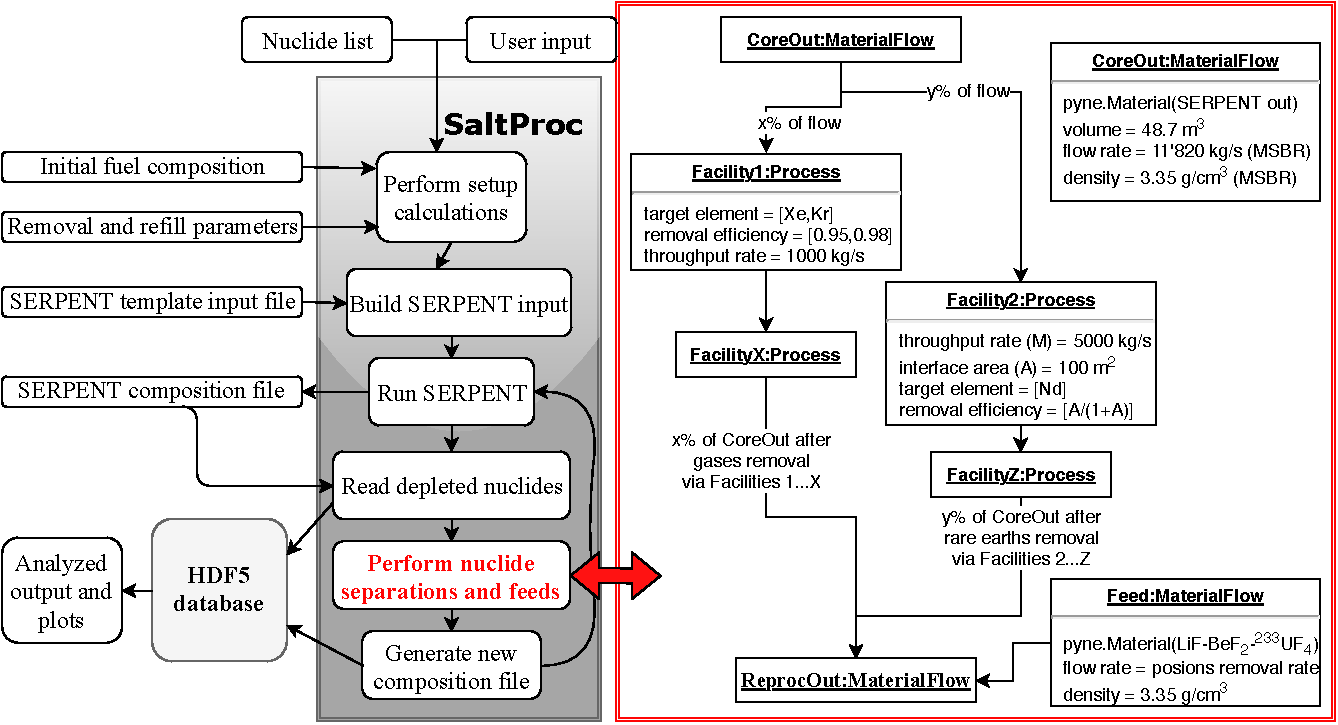
\includegraphics[width=1.05\textwidth]{saltproc_flowchart.pdf}
  \caption{Tentative generic flow chart for new Saltproc python package.}
  \label{fig:saltproc_flow}
\end{figure}

For a more general case with multiple concurrent extraction processes a separate 
\textit{MaterialFlow} object will be created for each branch with a user-defined 
mass flow rate (e.g. 90\% of total mass flow rate flows via left branch and 
10\% through right branch). Total volume and isotopic composition vector 
for each \textit{MaterialFlow} object will be calculated as a fraction of incoming 
\textit{CoreOut} flow. Then each \textit{MaterialFlow} object will be passed via 
a cascade of \textit{Processes} to separate selected chemical elements with 
specific efficiency. Finally, the left-hand-side branch \textit{MaterialFlow} object 
will be merged with the right-hand-side and similarly to previous case, fresh 
fuel salt feed will compensate the loss of mass in separation facilities and keep 
fuel salt mass in a primary loop constant.

The class diagram (Figure~\ref{fig:saltproc_class}) will allow simulating 
the operation of a complex, multi-zone, 
multi-fluid \gls{MSR} and is sufficiently general to represent myriad reactor 
systems. The refactored version of SaltProc will only store and edit the 
isotopic composition of the fuel stream, which makes it a flexible tool to 
model any geometry: an infinite medium, a unit cell, a multi-zone simplified 
assembly, or a full core. This flexibiliity allows the user to perform 
simulations of varying fidelity and computational intensity. SaltProc is an 
open-source tool (but a user needs SERPENT2 installed to use SaltProc), 
available on Github. It will leverage unit tests and continuous integration 
crucial for sustainable development. It will also have documentation
generated through Sphinx, a documentation generator, for ease of use. In summary, the 
development approach of SaltProc is focused on producing a generic, flexible and 
expandable tool to give the SERPENT 2 Monte Carlo code the ability to conduct 
advanced in-reactor fuel cycle analysis as well as simulate many 
online refueling and fuel reprocessing systems.

%\subsection{Reactivity control module}
%In addition, SaltProc will be able to define time-dependent material feed and 
%removal rates to investigate their impacts. These rates need not be 
%constant in SaltProc. They can be defined as piecewise functions or set to 
%respond to conditions in the core. For instance, SaltProc might increase the 
%fissile material feeding rate if the effective multiplication factor, 
%$k_{eff}$, falls below a specific limit (e.g., 1.002).
%These capabilities allow SaltProc to analyze fuel cycle of a generic 
%liquid-fueled \gls{MSR}.

